\section{Benchmarks with Trigonometric Dynamics}
In this section, we show the efficacy of dynamic strategies on more general sets of benchmarks other than ones restricted to polynomial dynamics. In particular, we wish to demonstrate the improvements reaped by utilizing \emph{Kodiak} over exclusively using Bernstein polynomials to perform the optimization shown in Equation~\ref{eq:maxf} above.

\subsection{Inverted Pendulum Model}
We test our strategies on the well-known Inverted Pendulum model governed by the following dynamics:
\begin{align}
  x' & = y \\
  y' & = -0.2y - \sin{x}
\end{align}
The model is run for 80 timesteps with discretization step $\Delta=0.1$. The initial set is set to be
\[ x \in [0.25, 0.3], \quad y \in [0.25, 0.3] \]
%
We present the same data and plots shown for the benchmarks with polynomial dynamics above.

\begin{figure}[h!]
  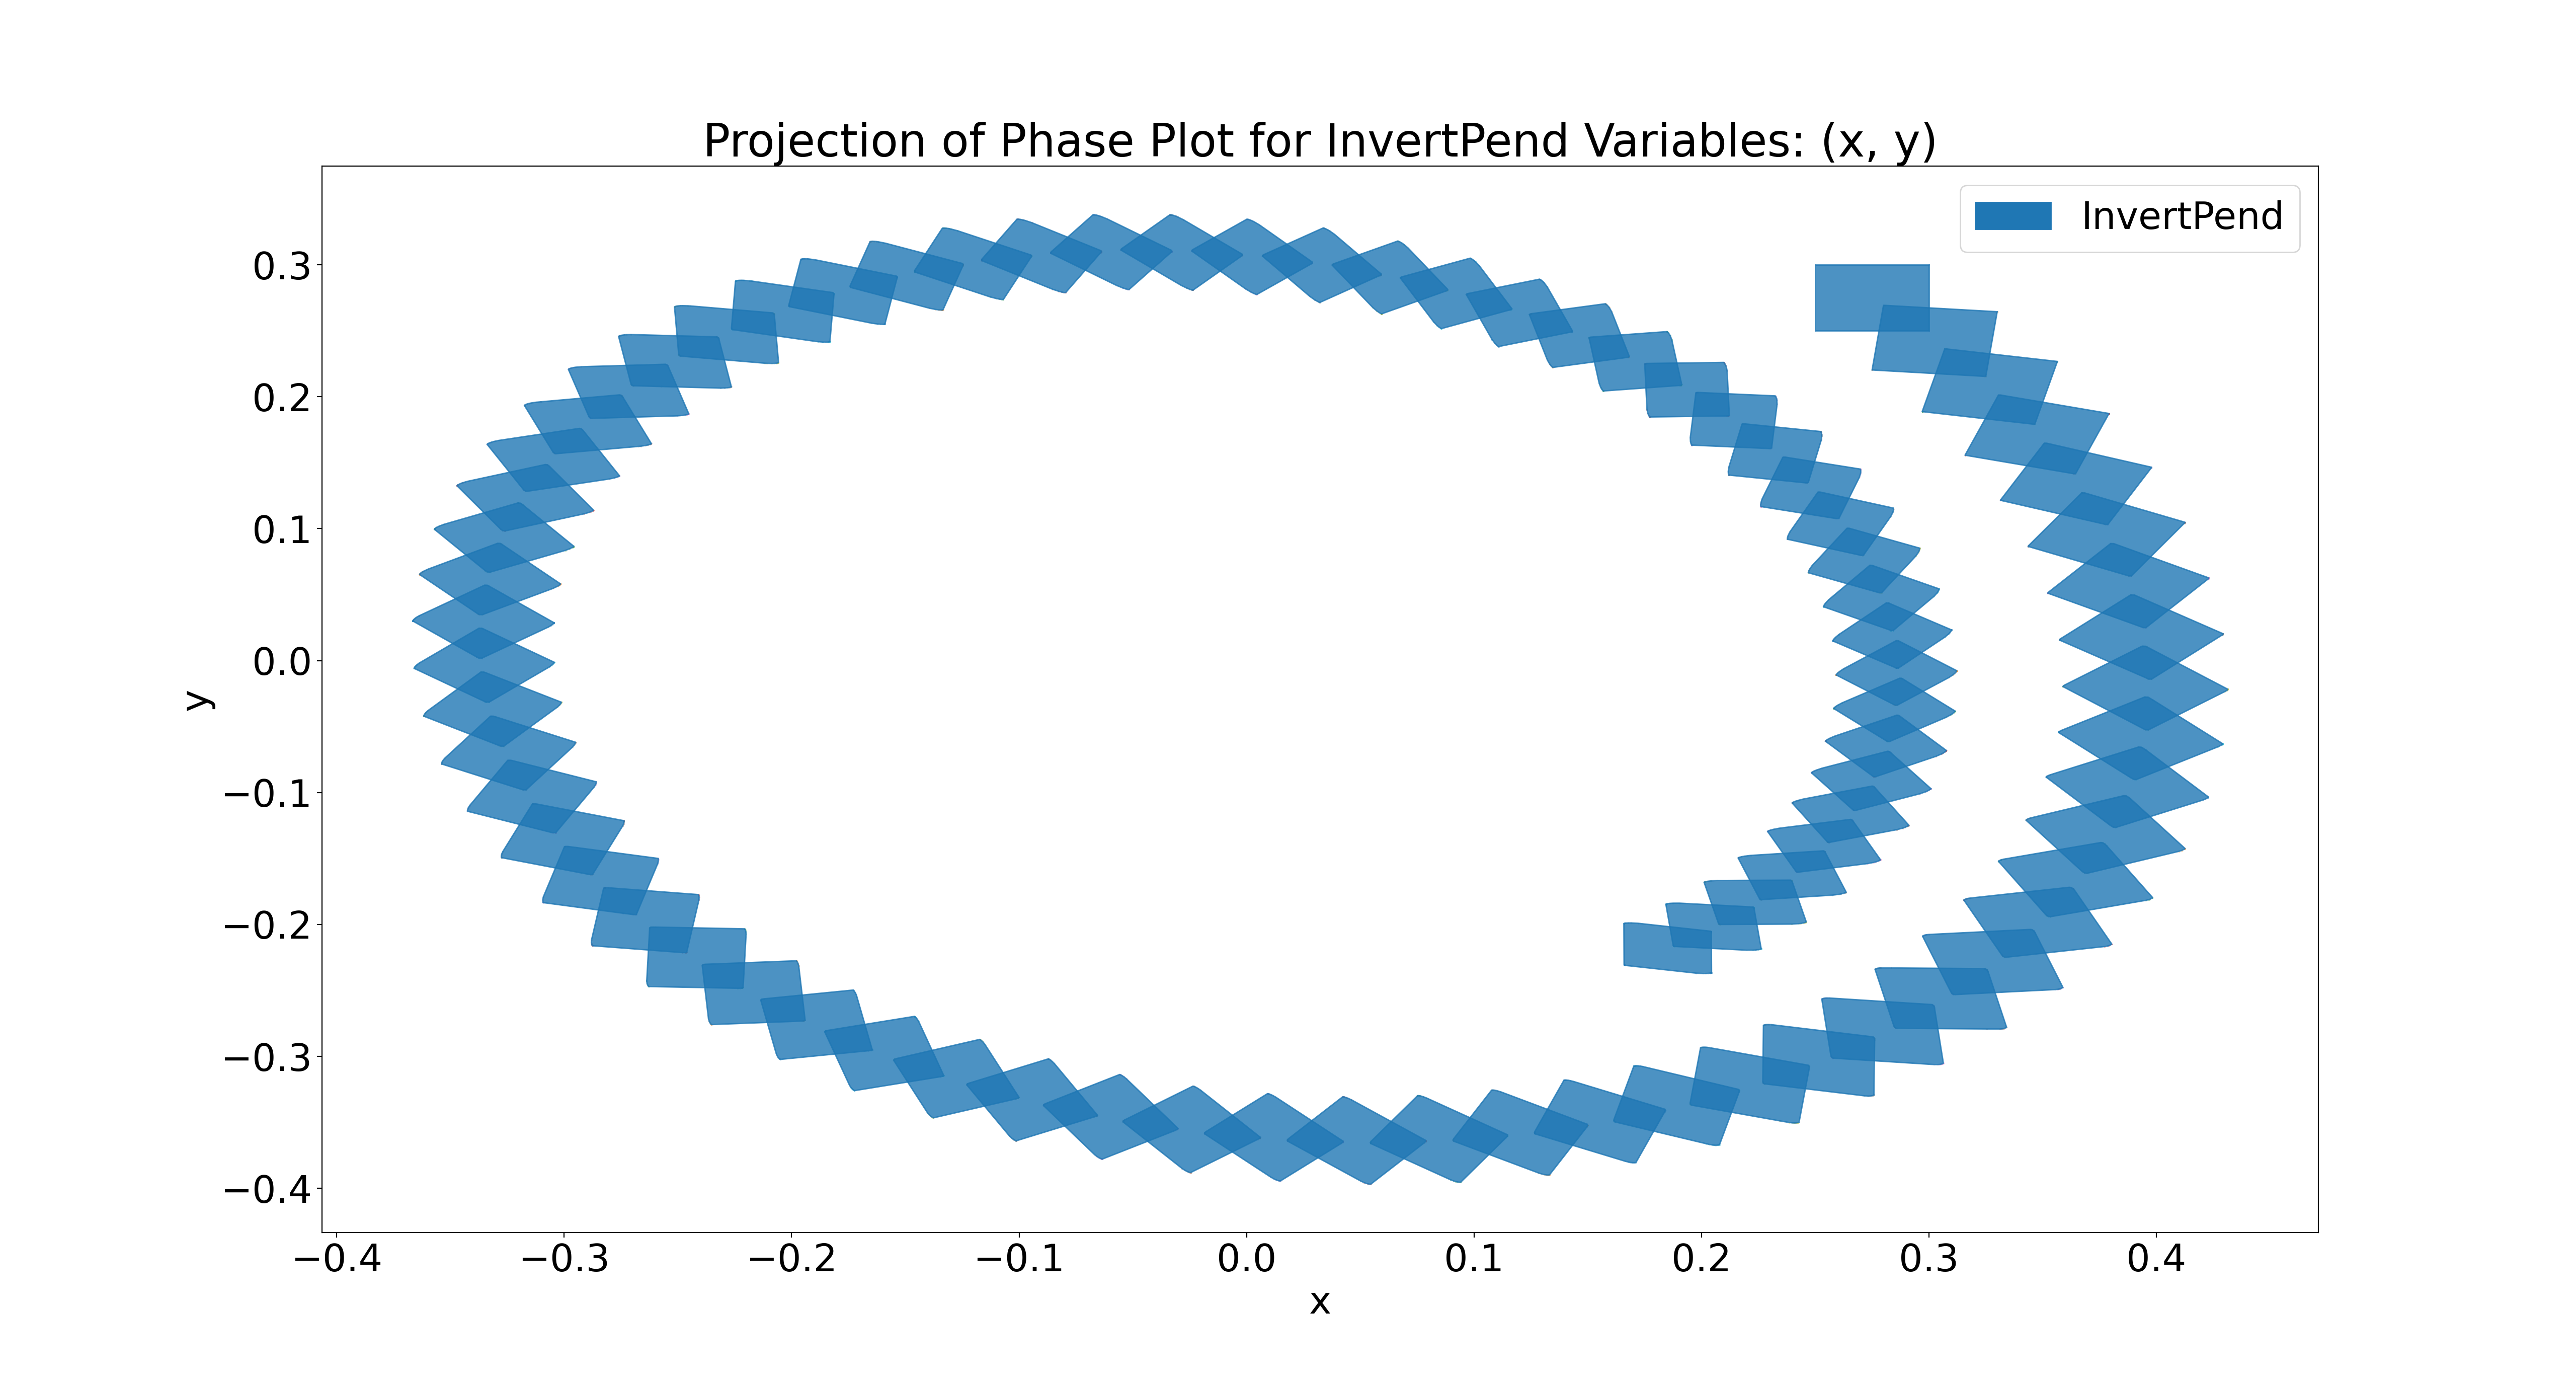
\includegraphics[width=\textwidth, height=0.75\textwidth]{figures/InvertPend}
  \caption{Reachable set for the Inverted Pendulum model executed under the parameters presented above.}
\end{figure}
